\documentclass[tikz,border=3.14pt]{standalone}
\usepackage{tikz}
\usetikzlibrary{arrows.meta}
\usepackage{amsmath}
\usepackage{physics}

\ExplSyntaxOn
\msg_redirect_name:nnn { siunitx } { physics-pkg } { none }
\ExplSyntaxOff

\begin{document}
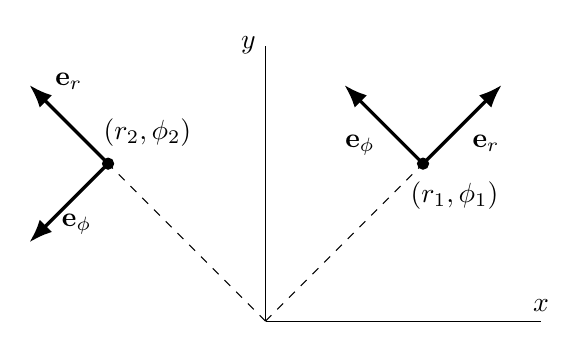
\begin{tikzpicture}[scale=2,
		vector/.style={-{Latex}, very thick}]

        \coordinate (P) at (1, 1);
        \coordinate (Q) at (-1, 1);

        \draw (0, 0) -- (1.75, 0) node [above, pos=1] {$x$};
        \draw (0, 0) -- (0, 1.75) node [left, pos=1] {$y$};

        \draw [dashed] (0, 0) -- (P);
        \draw [fill] (P) circle (1pt);
        \node at (1.2, 0.8) {$\left(r_{1}, \phi_{1} \right)$};
        \draw [vector] (P) -- ++(0.5, 0.5) node [pos=0.8, below=3mm] {$\vb{e}_{r}$};
        \draw [vector] (P) -- ++(-0.5, 0.5) node [pos=0.8, below=3mm] {$\vb{e}_{\phi}$};


        \draw [dashed] (0, 0) -- (Q);
        \draw [fill] (Q) circle (1pt);
        \node at (-0.75, 1.2) {$\left(r_{2}, \phi_{2} \right)$};
        \draw [vector] (Q) -- ++(-0.5, 0.5) node [pos=0.5, above=3mm] {$\vb{e}_{r}$};
        \draw [vector] (Q) -- ++(-0.5, -0.5) node [pos=0.4, below=1mm] {$\vb{e}_{\phi}$};
\end{tikzpicture}
\end{document}